\chapter{Inverse Kinematics}
\label{chap:inv kin}


\section{Introduction}

The goal of the robotics project is to control the movement of a 7 DOF robot arm with several joints.\\
The robot used for this project is the Baxter and the task that it has to execute is a drawing.


\section{Denavit-Hartenberg parameters}
\subsection{Theoretical calculation}
To be able to compute the inverse kinematics of a robot efficiently in a minimal and systematic way, the kinematics of the system can be described using Denavit-Hartenberg parameters. \\
Before doing this, it is important to note that Baxter has seven joints for each arm (which means 7 degrees of freedom) while a task in the real world 3D space needs only six degrees of freedom, namely three rotations and three translations. Therefore, the arms of Baxter have one redundant degree of freedom for general tasks.\\
Redundancy can be helpful for avoiding obstacles, increasing the range of the workspace or allow to reach a position and orientation by avoiding it nevertheless it adds complexity for the problem.\\
The group has chosen in this case to fix a joint, $E_0$ not represented in the Figure (\ref{fig:prios}) but present on the information on Baxter website.\footnote{\url{http://sdk.rethinkrobotics.com/wiki/Hardware\_Specifications}} \\

The first thing to do to calculate the DH parameters is to fix the frame of each joint. Some rules has to be respected: \\
\begin{itemize}
\item $z_{i-1}$ axis has to be along the axis of joint i
\item $x_{i-1}$ axis is along the common normal between joint axis i-1 and i
\end{itemize}

The origin is simply on the intersection of x and z and the y-axis can be found thanks to the right-hand rule.\\
However two specific cases still have to be defined: \\
\begin{itemize}
\item the origin and the $x_0$-axis are chosen freely
\item the $z_n$-axis is not specified ( but $x_n$ must be orthogonal to and intersect $z_{n-1}$ 
\item if $z_i$ and $z_{i-1}$ are parallel, the commono normal is not unique and then the origin $O_i$ can be chosen arbitrairly.
\item if $z_i$ and $z_{i-1}$ are incident, the positive direction of $x_i$ can be chosen arbitrairly ( however, it is often chosen so that $x_i = z_i$ x $z_{i-1}$)
\end{itemize}

 \begin{figure}[!ht]
	\centering
    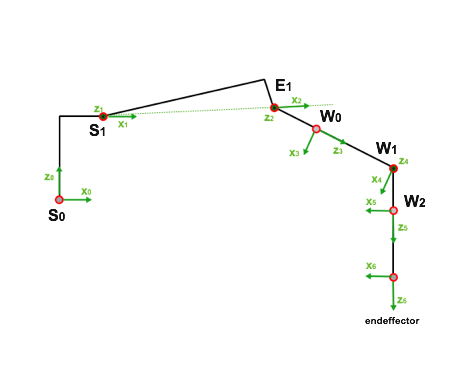
\includegraphics[width = 0.7\textwidth]{Images/DHparam}
    \caption{Schematic drawing of the Baxter arm for the determination of the DH parameters.}
    \label{fig:DHparam}
\end{figure}

The frames are now fixed, the DH parameters can then be calculated. \\
Rules have to be followed again:\\
\begin{itemize}
\item $a_i$ is the distance between the two points that intersect the joint axis $z_i$ and $z_{i+1}$ with their common normal
\item $d_i$ is the distance between the origin $O_i$ and the intersection between the joint axis $z_i$ and the common normal with joint axis $z_{i+1}$
\item $\alpha_i$ is the twist angle between the joint axis $z_i$ and $z_{i+1}$
\item $\theta_i$ is the angle between $x_{i-1}$ and $x_i$ around $z_{i-1}$
\end{itemize}

A summary of the determination of these parameters coming from the course.\footnote{Course of robotics of Michael Van Damme}

\begin{figure}[!ht]
	\centering
    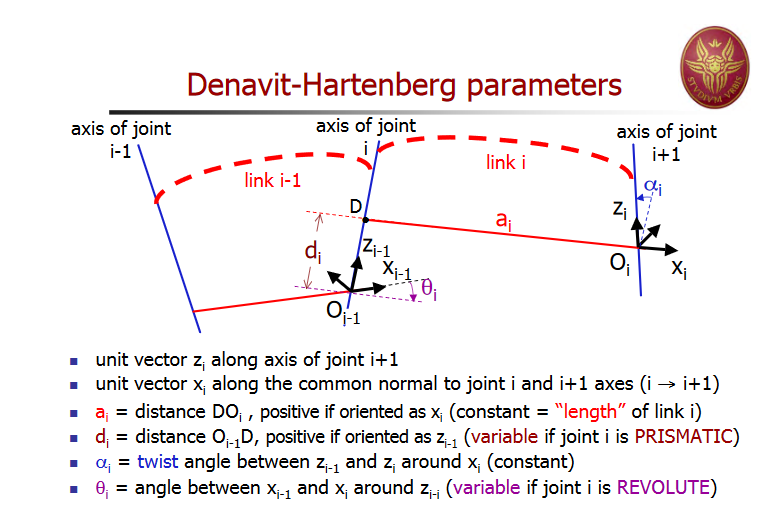
\includegraphics[width = 0.9\textwidth]{Images/DHparameters}
    \caption{Determination of DH parameters}
    \label{fig:DH}
\end{figure}

This parameters will allow to calculate the matrix defining the combination of the roto-translation around and along $x_{i-1}$ and $z_{i-1}$. \\

\begin{center}
	\begin{equation}
		A^{i-1}_{i}(q_i) = A^{i-1}_{i'}(q_i) * A^{i'}_{i}(q_i) = \begin{bmatrix}
		c\theta_i & -c\alpha_is\theta_i & s\alpha_is\theta_i & a_ic\theta_i \\
        s\theta_i & c\alpha_ic\theta_i & -s\alpha_ic\theta_i & a_is\theta_i \\
        0 & s \alpha_i & c \alpha_i & d_i\\
        0 & 0 & 0 & 1
		\end{bmatrix}
	\end{equation}
\end{center}


The matrix of a roto-translation can be represent as: \\
\begin{center}
	 \begin{equation}
	 	T^i_{i-1} = \begin{bmatrix}
	 	R & p\\ 0 & 1
	 	\end{bmatrix}
	 \end{equation}
\end{center}

Where R is a 3x3 matrix of rotation, p is a vector 3x1 representing the translation between $O_{i-1}$ and $O_i$, 0 is a null matrix 1x3 and 1 is simply a scalar.

\subsection{Result of DH parameters}

The values of the parameters is represented in a table.\\

\begin{center}
	\begin{tabular}{c|c c c c }

		Joint & $a_i$ & $d_i$ & $\alpha_i$  & $\theta_i$ \\
        \hline
        $S_0$ & 69 & 270.35 & $\pi$ /2 & $\theta_1$ \\
        $S_1$ & 370.82 & 0 & 0 & $\theta_2$ + $\beta$\\
        $E_1$ & 0 & 0 & - $\pi$/2 & $\theta_3$ + $\pi$ + $\beta$\\
        $W_0$ & 10 & 374.29 & $\pi/2$ & $\theta_4$\\
        $W_1$ & 0 & 0 & - $\pi$ /2 & $\theta_5$ \\
        $W_2$ & 0 & 229.525 & 0 & $\theta_6$
	\end{tabular}
\end{center}

Where $\beta$ is $arctg(\frac{69}{364.35})$ or $10,7^\circ$.


\section{Task Description}
The calculations for the inverse kinematics can be simplified based on the tasks that will have to be executed. This will allow to fix some degrees of freedom, or some relationships between the joint angles.\\
\noindent The task that the robot will execute is the following: the robot will pick a paint brush, dip it in a cup with some acrylic paint, draw a circle on a sheet of paper and then place the brush in a cup of water. To calibrate the orientation of the paper sheet at the beginning of the execution, to robot arm will first point to two reference points, which will have to correspond to those shown in Figure \ref{fig:Task}. The robot will then bring the brush to the consecutive waypoints, which all have their specific coordinates.


\begin{figure}[!ht]
	\centering
    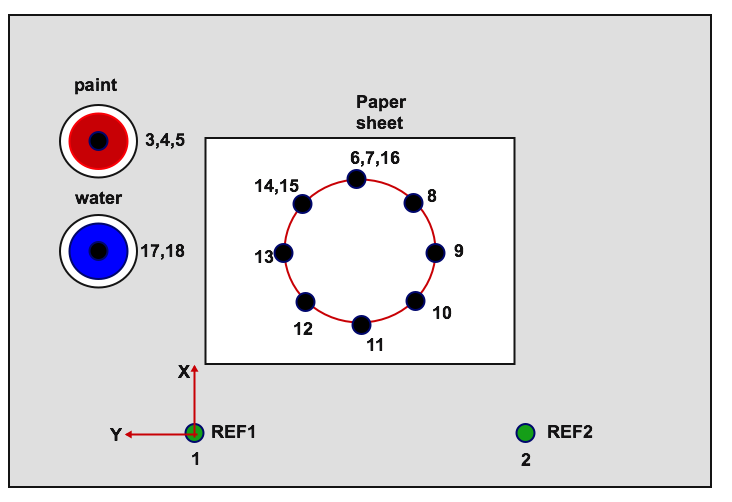
\includegraphics[width = 0.6\textwidth]{Images/Task}
    \caption{Projection of the waypoints describing the task on the X-Y plane, which corresponds to the table surface.}
    \label{fig:Task}
\end{figure}

\bigskip
A first observation is that the last link in the kinematic chain can stay in a vertical position during the whole execution process. Also, the paint brush does not have to rotate around the vertical axis, so that joint W2 can be fixed. Since it is assumed that there are no specific constrains for the workspace of the robot arm, there are still some redundant degrees of freedom that will not be used. Therefore, joint W0 can also be fixed. Further developments will be discussed in


\section{Inverse kinematics}
\label{sec: inv}
The equations for the inverse kinematics can be complicate so the group has try to simplify them as much as possible.\\
The six remaining joints of the robot can be divided in two parts. The three last joint correspond to a spherical wrist and so will focus on the orientation of the end-effector while the three other joints will be used to put the end-effector at the right position.\\

The task that will make the robot is a drawing. In this case the paintbrush has to be all the time perpendicular to the table. So the joint $W_0$ has to be fixed to 0 for that the arm of the robot moves only in a plane and the joint $W_1$ has to compensate joint $S_1$ and $E_1$ so that $z_5$ is parallel to $z_0$. The $90^{\circ}$ between $S_1$ and $E_1$ has to be taken into account and that if the angles of all the joints are zero, the arm is parallel to the ground.\\
It is now easy to see than $\theta_5 = \pi /2 - (\theta_1 + \theta_2)$. \\
The last joint has no importance in our case, it has been fixed arbitrarily to zero.\\

The position of the robot still has to be calculated. The position of the end-effector will be evaluated based on the wrist point and the rotation between the first and the last frames. \\

\begin{center}
	\begin{equation}
		p^0_e = p^0_w + d_6 z ^0_6 = p^0_w + d_6 R_e^0 \begin{vmatrix}
		0 \\ 0 \\ 1
		\end{vmatrix}
	\end{equation}
\end{center}

\begin{center}
	\begin{equation}
		p^0_w = p^0_e - d_6 R_e^0 \begin{vmatrix}
		0 \\ 0 \\ 1
		\end{vmatrix}
	\end{equation}
\end{center}

Where $d_6^0$ is the distance between the wrist point and the end-effector and $R^0_e$ is the rotation between frame 0 and frame 6.\\
The arm being perpendicular to the table, the difference between the wirst point and the end-effector is simply a difference of height that correspond to 270.35 - 229.525. \\


For the calculation of the position to reach, the raisonning looks like one example made during the course.\\
The angle $\theta1$ correspond to the orientation of the arm. It is calculated thanks to the x and y that will be given using the equation of trigonometry.\\

\begin{center}
	\begin{equation}
		\theta_1 = Atan2(y_c,x_c)
	\end{equation}
\end{center}

\noindent The function Atan2 allows to have a angle between - $\pi$ and $\pi$ instead of between 0 and $\pi$.\\

\noindent The two last angles are slightly more difficult to calculate.\\

\begin{figure}[!ht]
	\centering
    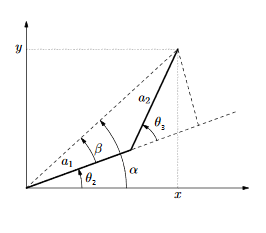
\includegraphics[width = 0.7\textwidth]{Images/angles}
    \caption{Calculation of $\theta_2$ and $\theta_3$}
    \label{fig:angles}
\end{figure}

The angle $\pi - \theta_3$ is found thanks to Pythagore.\\

\begin{center}
	\begin{equation}
		x^2 + y^2 = a_1^2 + a_2^2 - 2a_1a_2cos(\pi - \theta_3) = a_1^2 + a_2^2 + 2a_1a_2cos(\theta_3)
	\end{equation}
\end{center}

\begin{center}
	\begin{equation}
		cos(\theta_3) = \frac{x^2 + y^2 - a_1^2 - a_2^2}{2a_1a_2}
	\end{equation}
\end{center}

To be able to use the function Atan2, the sine of the angle is also need:\\

\begin{center}
	\begin{equation}
		sin(\theta_3) = \sqrt{1 - (cos(\theta_3))^2}
	\end{equation}
\end{center}

So: \\

\begin{center}
	\begin{equation}
		\theta_3 = Atan2(sin(\theta_3),cos(\theta_3))
	\end{equation}
\end{center}

The base of the calculation is $\theta_2$ equals $\alpha$ minus $\beta$.\\
The calculation of $\alpha$ is the same than for $\theta_1$ and the calculation of $\beta$ is made thanks to the triangle in dashed line.\\

\begin{center}
	\begin{equation}
		tg(\beta) = \frac{a_2sin(\theta_3)}{a_1+cos(\theta_3)}
	\end{equation}
\end{center}

So $\theta_2$ is:\\

\begin{center}
	\begin{equation}
		\theta_2 = Atan2(y,x) - Atan2(a_2sin(\theta_3),a_1+cos(\theta_3))
	\end{equation}
\end{center}